\documentclass[tikz,border=8pt]{standalone}
% Shared look for every TikZ diagram. Load with \input{../../tools/tikz-style.tex}
\usepackage[T1]{fontenc}
\usepackage{lmodern}
\renewcommand{\sfdefault}{lmr}  % diagrams use the same serif as the text
\usetikzlibrary{arrows.meta, positioning, shapes.geometric, calc, fit, backgrounds}
\definecolor{cblue}{HTML}{4C78A8}
\definecolor{corange}{HTML}{F58518}
\definecolor{cgreen}{HTML}{54A24B}
\definecolor{cred}{HTML}{E45756}
\definecolor{cpurple}{HTML}{B279A2}
\definecolor{cgrey}{HTML}{6B6B6B}
\tikzset{
  every picture/.style={font=\sffamily, line width=1.2pt},
  box/.style={draw=#1, fill=#1!12, rounded corners=4pt, align=center, inner sep=7pt, minimum height=1.1cm},
  box/.default=cgrey,
  arrow/.style={-{Stealth[length=3mm]}, draw=cgrey, line width=1.4pt},
  title/.style={font=\sffamily\bfseries\Large},
  note/.style={font=\sffamily\small, text=cgrey, align=center},
}
\AtBeginDocument{\hyphenpenalty=10000 \exhyphenpenalty=10000}

% A guessed pose C = (3.9, 2, -90 deg) above the box. A reading of 1.98 m would end at (3.9, 0.02), right next to
% the bottom wall, so the likelihood field scores it high (3.45 per m). But the beam would have to pass through
% the box, which starts 0.8 m below C; the beam model gives it only 0.016 per m.
\begin{document}
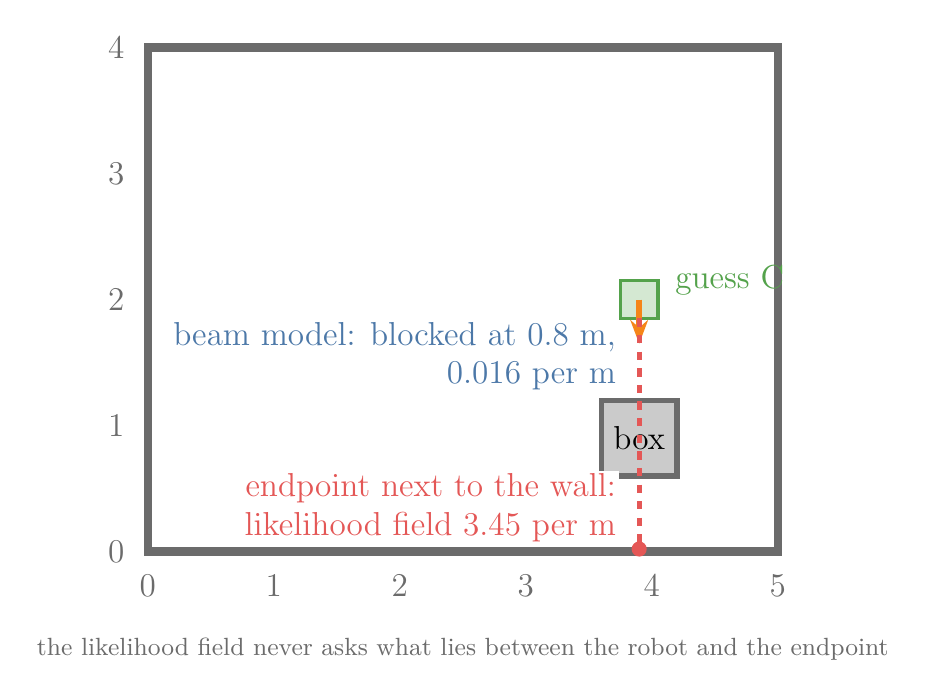
\begin{tikzpicture}[scale=1.6, every node/.append style={font=\large}]
  \draw[cgrey, line width=3pt] (0,0) rectangle (5,4);
  \draw[cgrey, fill=cgrey!35, line width=2pt] (3.6,0.6) rectangle (4.2,1.2);
  \node at (3.9,0.9) {box};
  \foreach \x in {0,1,...,5} \node[below, cgrey] at (\x,-0.1) {\x};
  \foreach \y in {0,1,...,4} \node[left, cgrey] at (-0.1,\y) {\y};
  \draw[cgreen, fill=cgreen!25] (3.75,1.85) rectangle (4.05,2.15);
  \draw[-{Stealth[length=3mm]}, corange, line width=2pt] (3.9,2) -- (3.9,1.65);
  \node[cgreen, right] at (4.1,2.15) {guess C};
  \draw[cred, line width=1.8pt, dashed] (3.9,1.85) -- (3.9,0.02);
  \fill[cred] (3.9,0.02) circle (0.06);
  \node[cred, left, fill=white, inner sep=1pt, align=right] at (3.75,0.35) {endpoint next to the wall:\\ likelihood field $3.45$ per m};
  \node[cblue, left, fill=white, inner sep=1pt, align=right] at (3.75,1.55) {beam model: blocked at $0.8$ m,\\ $0.016$ per m};
  \node[note, anchor=north] at (2.5,-0.6) {the likelihood field never asks what lies between the robot and the endpoint};
\end{tikzpicture}
\end{document}
